%%% Dateikodierung: UTF-8

%%% Magic Comments zum Setzen der korrekten Parameter in kompatiblen IDEs
% !TeX encoding = utf8
% !TeX program = pdflatex 
% !TeX spellcheck = de_DE
% !BIB program = biber

\RequirePackage[utf8]{inputenc} % bei Verw. von lualatex oder xelatex entfernen!
\RequirePackage{hgbpdfa}        % Erzeugt ein PDF/A-2b-konformes Dokument

\documentclass[type=bachelor, theme=default, language=german, titlelanguage=german, smartquotes, notitlepage, nodeclaration]{hgbthesis}
\usepackage{pdfpages}
\setlength{\parindent}{0pt}

\graphicspath{{images/}}  % Verzeichnis mit Bildern und Grafiken
\bibliography{references} % Biblatex-Literaturdatei (references.bib)

%%%-----------------------------------------------------------------------------
\begin{document}
%%%-----------------------------------------------------------------------------

%%%-----------------------------------------------------------------------------
\frontmatter                                       % Titelei (röm. Seitenzahlen)
%%%-----------------------------------------------------------------------------

\setcounter{page}{-1}

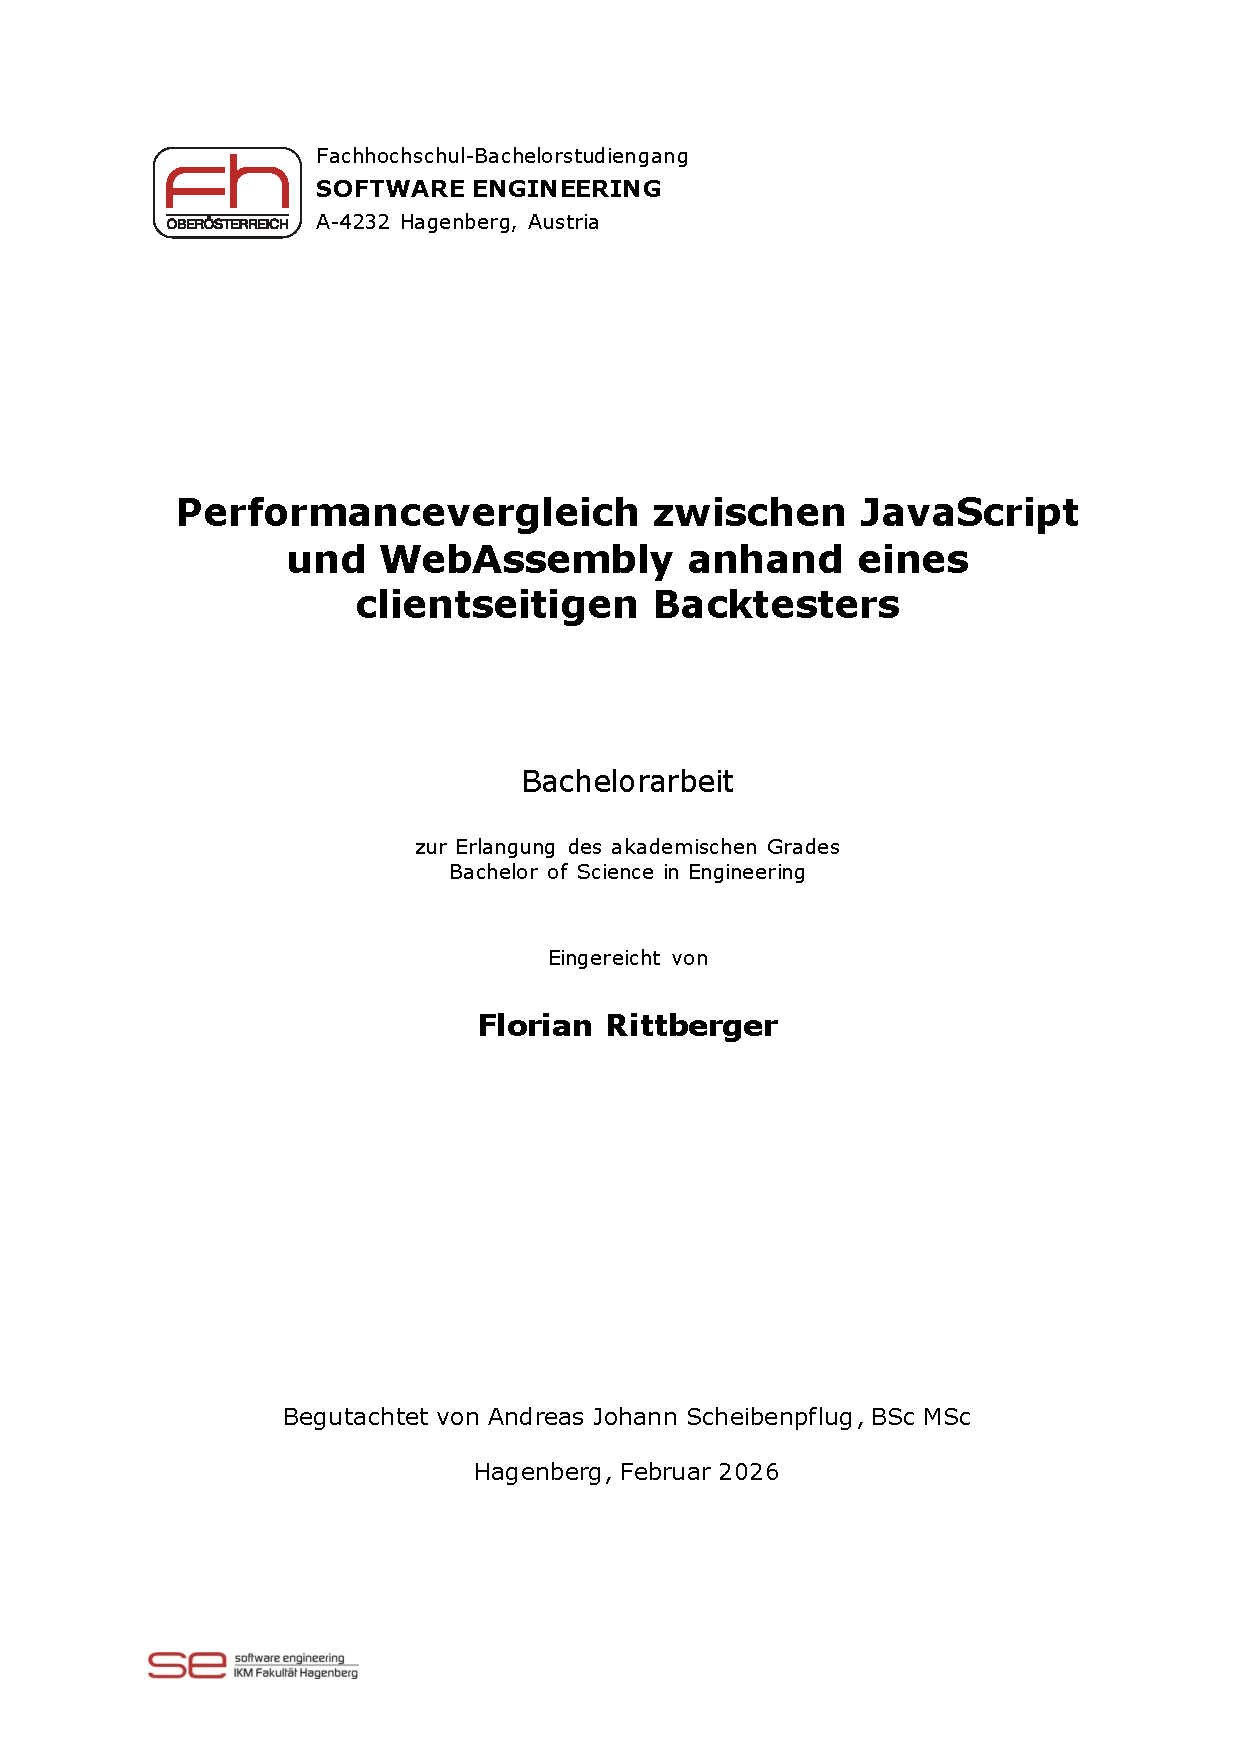
\includepdf[pages=1-2, pagecommand={}, fitpaper=true]{./pdf/Titelblattvorlage_Bachelorarbeit.pdf}

\setcounter{page}{1}

\tableofcontents

\chapter{Kurzfassung}

\begin{german}
In dieser Arbeit wird die Performanz von WebAssembly und JavaScript verglichen.
Der Vergleich wird mit einem clientseitigen Backtester durchgeführt, der Handelsstrategien in beiden Sprachen unterstützt.
Ein Backtester ist eine Software mit der Handelsstrategien anhand historischer Kursdaten getestet werden können.
Strategien sind Algorithmen, die automatisch Kauf- und Verkaufsentscheidungen treffen, um Gewinne zu erzielen, ohne selbst aktiv handeln zu müssen.
Der Backtester ist ein geeignetes Programm zum Vergleich der beiden Programmiersprachen, da der Prozess des Backtestings rechenintensiv ist und somit die Performanzunterschiede gut erkennbar sind.
\newline

Der Backtester wird als Webanwendung in JavaScript implementiert, die im Browser ausgeführt wird.
Für den Vergleich der Sprachen wird der rechenaufwendigste Teil des Backtestings, die Strategien, ausgelagert und in WebAssembly und JavaScript implementiert.
Damit die Ausführungszeiten bei unterschiedlichem Rechenaufwand verglichen werden können, werden drei unterschiedliche Handelsstrategien mit steigender Komplexität implementiert.
Die entwickelten Strategien sind eine Gleitende Durchschnitts Überscheidungsstrategie, eine Ausbruchsstrategie und eine Mittelwertrückkehrstrategie mit Bollinger Bänder.
Anhand dieser Strategien kann die Performanz und Varianz von JavaScript und WebAssembly verglichen werden.
\newline

Durch die Tests der Strategien mit verschiedenen Datensätzen ist erkennbar, dass WebAssembly in Firefox bei rechenintensiven Strategien schneller ist als JavaScript.
Ebenfalls ist die Varianz der durchschnittlichen Ausführungszeiten von WebAssembly in Firefox geringer als die von JavaScript.
In Chrome hingegen ist JavaScript bei jeder getesteten Strategie schneller als WebAssembly.
Die Varianz ist in Chrome bei WebAssembly geringer als bei JavaScript.
Insgesamt ist zu erkennen, dass die Performanz von WebAssembly und JavaScript vom verwendeten Browser und der Rechenintensität der Strategie abhängt.
Jedoch kann WebAssembly bei rechenintensiven Aufgaben einen großen Vorteil in der Ausführung bieten.
\end{german}		
\chapter{Abstract}

\begin{english}
This paper compares the performance of WebAssembly and JavaScript.
The comparison is made with a clientside backtester that supports trading strategies in both languages.
A backtester is a software that allows the testing of trading strategies based on historical price data.
Strategies are algorithms that automatically make buying and selling decisions in order to make profits without active interaction.
The backtester is a suitable program for comparing the two programming languages, because the backtesting process is very computationally intensive and thus the performance differences are clearly visible.
\newline

The backtester is implemented as a web application in JavaScript that runs in the browser.
To compare the languages, the most computationally intensive part of backtesting, the strategies, is outsourced and implemented in WebAssembly and JavaScript.
To be able to compare the execution times at different computational loads, three different trading strategies with increasing complexity are implemented.
The developed strategies are a moving average crossover strategy, a breakout strategy and a mean reversion strategy with Bollinger bands.
Because of these strategies, the performance and variance of JavaScript and WebAssembly can be compared.
\newline

Overall, it can be seen that the performance of WebAssembly and JavaScript depends on the browser used and the computational intensity of the strategy.
However, WebAssembly can offer a significant advantage in execution for computationally intensive tasks.
Testing the strategies with different data sets shows that WebAssembly in Firefox is faster than JavaScript for computationally intensive strategies.
Furthermore, the variance in the average execution times for WebAssembly in Firefox is lower than that for JavaScript.
In Chrome, on the other hand, JavaScript is faster than WebAssembly for every strategy tested.
The variance in Chrome is lower for WebAssembly than for JavaScript.
\end{english}



%%%-----------------------------------------------------------------------------
\mainmatter                             % Hauptteil (ab hier arab. Seitenzahlen)
%%%-----------------------------------------------------------------------------

\chapter{Einleitung}
\label{cha:Einleitung}

Wenn man automatisiert handeln möchste braucht man eine Stragie. Zum testen braucht man auch etwas. Den Backtester.
Arbeit wird ein Backtster entwickelt. Der clientseitig ist. Weniger Sicherheitslücken. Doch wie ist der Backtester am schnellsten.
Deswegen rechenintenveste Teil ausgelagert. Die Strategien. Diese mit neuen Web Technologien wie WASM im Vergleich zu reinem JS.
Nur diese 1 Seite

\section{Motivation der Arbeit}
\label{sec:MotivationderArbeit}

\section{Ziele der Arbeit}
\label{sec:ZielederArbeit}

\section{Vorgangsweise zur Zielerreichung}
\label{sec:VorgangsweisezurZielerreichung}

\section{Kapitelübersicht}
\label{sec:Kapitelübersicht}

In diesem Unterkapitel werden die einzelnen Kapitel überblicksmäßig beschrieben.

\subsection{Grundlegende Konzepte und Technologien}
\label{subsec:GrundlegendeKonzepteundTechnologien}

In dem Kaptiel \ref{cha:GrundlegendeKonzepteundTechnologien} werden die Grundlagen und die relevanten Technologien beschrieben.
Dabei werden die grundlegenden Themen wie Backtesting, Biase im Backtesting, bereits existierende Backtester sowie Ansätze für Handelsstrategien näher erläutert.
Zudem wird WebAssembly als eine der Kerntechnologien vorgestellt und wie diese in Webanwendungen integriert wird.

\subsection{Konzept und Design}
\label{subsec:KonzeptundDesign}

Das Kaptiel \ref{cha:KonzeptundDesign} beschreibt wie die einzelnen Komponenten des entwickelten Backtester aufgebaut sind, wie die Geschwindigkeitstests durchgeführt werden und welche Werkzeuge für die Entwicklung von WebAssembly genutzt wurden. 

\subsection{Implementierung des Backtesters und der Strategien}
\label{subsec:ImplementierungdesBacktestersundderStrategien}

In dem Kaptiel \ref{cha:ImplementierungdesBacktestersundderStrategien} wird die Implementierung des Backtesters und der Handelsstrategien beschrieben.
Dabei wird der gesamte Prozess von der Beschaffung historischer Daten über das Laden und Anwenden der Handelsstrategien bis hin zur Darstellung der Ergebnisse auf der Webseite beschrieben.

\subsection{Performanztests der unterschiedlichen Programmiersprachen}
\label{subsec:PerformanztestsderunterschiedlichenProgrammiersprachen}

Das Kaptiel \ref{cha:PerformanztestsderunterschiedlichenProgrammiersprachen} zeigt den Aufbau und die Ergebnisse der Performanztests der verschiedenen Implementierungen der Handelsstrategien in unterschiedlichen Programmiersprachen.
Es werden Strategien in verschiedene Programmiersprachen implementiert und deren Ausführungszeiten im Backtester in verschiedenen Browsern gemessen.
Desweitern werden die Ergebnisse der Performanztests analysiert und interpretiert.

\subsection{Zusammenfassung und Schlussbemerkungen}
\label{subsec:Zusammenfassung und Schlussbemerkungen}

Im Kapitel \ref{cha:ZusammenfassungundSchlussbemerkungen} wird die Arbeit zusammengefasst, ein Ausblick auf mögliche zukünftige Arbeiten gegeben und abschließend Erfahrungen einbezogen.

\include{chapters/grundlagen}
\include{chapters/konzept_und_design}
\chapter{Implementierung des Backtesters und der Strategien}
\label{cha:ImplementierungdesBacktestersundderStrategien}

In diesem Kapitel wird beschrieben wie die einzelnen Komponenten des Backtester und die getesteten Strategien implementiert sind.
\iffalse
\begin{CCode}[caption={Simple C example}, label={lst:c-example}]
#include <stdio.h>

int main(void)
{
    printf("Hello, world!\n");
    return 0;
}
\end{CCode}

\begin{HtmlCode}[caption={Basic HTML page}, label={lst:html-example}]
<!DOCTYPE html>
<html lang="en">
<head>
    <meta charset="UTF-8">
    <title>Example</title>
</head>
<body>
    <h1>Hello World</h1>
    <p>This is an HTML example.</p>
</body>
</html>
\end{HtmlCode}

\begin{JsCode}[caption={JavaScript example}, label={lst:js-example}]
function greet(name) {
    console.log(`Hello, ${name}!`);
}

greet("Alice");
\end{JsCode}
\fi

\section{Die Benutzerschnittstellen}
\label{sec:DieBenutzerschnittstellen}

\subsection{Die API Schnittstelle}
\label{subsec:DieAPISchnittstelle}

\subsection{Die Logikeingangsparameter}
\label{DieLogikeingangsparameter}

\section{Implementierung der Backtestlogik}
\label{sec:ImplementierungenderBacktestlogik}

\section{Implementierungen der Strategien}
\label{sec:ImplementierungenderStrategien}

Es werden drei verschiedene Handelsstrategien implementiert. Jede Strategie hat eine unterschiedliche Logik, um Kauf- und Verkaufsentscheidungen zu treffen.
Diese Unterschiede in der Logik führen zu unterschiedlichen Laufzeitkomplexitäten.
Die Ideen hinter den implementierten Strategien sind in Kapitel \ref{sec:Bewährte AnsätzefürHandelsstrategien} beschrieben.

Jede der folgenden Untersektionen beschreibt die Implementierung einer der drei Strategien in JavaScript und C.

\subsection{Gleitende Durchschnittsüberschneidungs Strategie}
\label{subsec:GleitendeDurchschnittsüberschneidungsStrategie}

\begin{CCode}[caption={Durchschnittsüberschneidung in C}, label={lst:DurchschnittsüberschneidunginC}]
    for (int i = prices_length - 1 - shortPeriod; i < prices_length - 1; i++) {
        shortPrev += prices[i];
    }
    shortPrev /= shortPeriod;

    for (int i = prices_length - 1 - longPeriod; i < prices_length - 1; i++) {
        longPrev += prices[i];
    }
    longPrev /= longPeriod;

    double shortCurr = 0.0;
    double longCurr = 0.0;

    for (int i = prices_length - shortPeriod; i < prices_length; i++) {
        shortCurr += prices[i];
    }
    shortCurr /= shortPeriod;

    for (int i = prices_length - longPeriod; i < prices_length; i++) {
        longCurr += prices[i];
    }
    longCurr /= longPeriod;

    const double diffPrev = shortPrev - longPrev;
    const double diffCurr = shortCurr - longCurr;

    double absDiff = diffCurr < 0.0 ? -diffCurr : diffCurr;

    const double currentPrice = prices[prices_length - 1];
    const double threshold = currentPrice * 0.002;

    if (diffPrev < 0.0 && diffCurr > 0.0 && absDiff >= threshold) {
        return 1;
    }
    if (diffPrev > 0.0 && diffCurr < 0.0 && absDiff >= threshold) {
        return -1;
    }
\end{CCode}

\subsection{Mittelwertrückkehr Strategie}
\label{subsec:MittelwertrückkehrStrategie}

\begin{CCode}[caption={Mittelwertrückkehr in C}, label={lst:MittelwertrückkehrinC}]
    double upperBand = mean + 3.25 * stdDev;
    double lowerBand = mean - 3.25 * stdDev;

    double lastPrice = prices[length - 1];

    if (lastPrice < lowerBand) {
        return 1;
    }
    if (lastPrice > upperBand) {
        return -1;
    }
\end{CCode}

\subsection{Ausbruchsstrategie}
\label{subsec:Ausbruchsstrategie}

\begin{CCode}[caption={Ausbruchsstrategie in C}, label={lst:AusbruchsstrategieinC}]
    double lastPrice = prices[length - 1];
    double epsilon = 0.01;

    double longTrigger = max * (1.0 + epsilon);
    double shortTrigger = min * (1.0 - epsilon);

    if (lastPrice > longTrigger) {
        return 1;
    }
    if (lastPrice < shortTrigger) {
        return -1;
    }
\end{CCode}

\section{Die Datenvisualisierungen}
\label{sec:DieDatenvisualisierungen}

\subsection{Visualisierung des Kurswertes}
\label{subsec:VisualisierungdesKurswertes}

\subsection{Visualisierung des Portfoliowertes}
\label{subsec:VisualisierungdesPortfoliowertes}
\include{chapters/performancetests_der_unterschiedlichen_programmiersprachen}
\chapter{Zusammenfassung und Schlussbemerkungen}
\label{cha:ZusammenfassungundSchlussbemerkungen}

In diesem Kapitel wird die Arbeit zusammengefasst, ein Ausblick auf mögliche zukünftige Erweitungen und Verbesserungen des Backtesters gegeben.

\section{Zusammenfassung}
\label{sec:Zusammenfassung}

\section{Ausblick und mögliche Erweiterungen des Backtesters}
\label{sec:AusblickundmöglicheErweiterungendesBacktesters}

Der in dieser Arbeit entwickelte Backtester bietet eine Grundlage für den Vergleich der Ausführungszeiten von WebAssembly und JavaScript und ermöglicht es Strategien mit einem Backtest zu analysieren.
Der Backtester kann zukünftig erweitert und angepasst werden, um weitere Funktionalität und Auswertungsmöglichkeiten zu bieten.
\newline
Spesen für Handel miteinbeziehen
Mehr paramter
\newline
Eine Verbesserungen wäre die Möglichkeit, mehrere Strategien und Datensätze gleichzeitg zu testen.
Somit können mit einem Durchlauf mehrere Testfälle gleichzeitg und benutzerfreundlicher angewandt werden.
Es müsste nicht mehr für jede Strategie und jeden Datensatz ein einzelner Test durchgeführt werden.
\newline
Die Berechung in Webworker auslagern.
\newline
Andere und genuere Statiken.
\newline
Download der Ergebnisse

%%%-----------------------------------------------------------------------------
\backmatter                          % Schlussteil (Quellenverzeichnis und dgl.)
%%%-----------------------------------------------------------------------------

\MakeBibliography % Quellenverzeichnis
\listoffigures
\listoftables
\lstlistoflistings

%%%-----------------------------------------------------------------------------
\end{document}
%%%-----------------------------------------------------------------------------
